{
\begin{table}\small
\begin{center}
\begin{tabular}{ p{1.2in} | p{1in} |p{1in} }    
 & \textbf{Logic} & \textbf{Memory} \\    
\textbf{Module} & \textbf{(LUT)} & \textbf{(BRAM)} \\    
\hline    
\hline    
%Firewall     & 2.8\% & 0.5\% \\    
%AES-256       & 0.4\% & 0 \\    
%Transport    & 1.3\% & 0.42\% \\    
%\hline
%\hline 
\snic{} Core & 4.36\%   & 4.74\% \\ 
Packet Store & 0.91\%   & 9.17\% \\
PHY+MAC      & 0.72\%   & 0.35\% \\
DDR4Controller         & 1.57\%   & 0.29\% \\
MicroBlaze   & 0.25\%   & 1.81\% \\
Misc         & 1.52\%   & 0.75\% \\
%\textbf{Total (w/o \nt{})}        & \textbf{9.33\%}   & \textbf{17.11\%} \\
\hline
\textbf{Total}        & \textbf{9.33\%}   & \textbf{17.11\%} \\    
    
\end{tabular}    
\mycaption{fig-fpga-resource}{SuperNIC FPGA Utilization.}    
{    
Shell cost in an FPGA. Most resources left for running \nt{}s.    
}
\end{center}
\end{table}
}
{
\begin{figure*}[t]
\begin{center}
\centerline{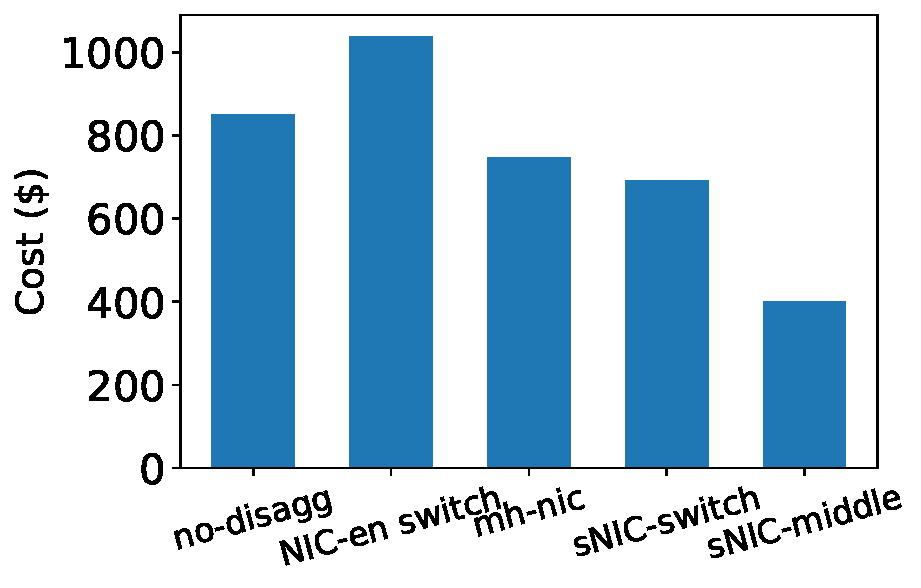
\includegraphics[width=0.5\textwidth]{snic/Figures/fig-single-rack-capex-perDevCost.pdf}}
\mycaption{fig-rack-capex}{Per-Endpoint CapEx.}
{
A rack's network cost divided by endpoint count. 
}
\end{center}
\end{figure*}
}
{
\begin{figure*}[h]
\begin{center}
\centerline{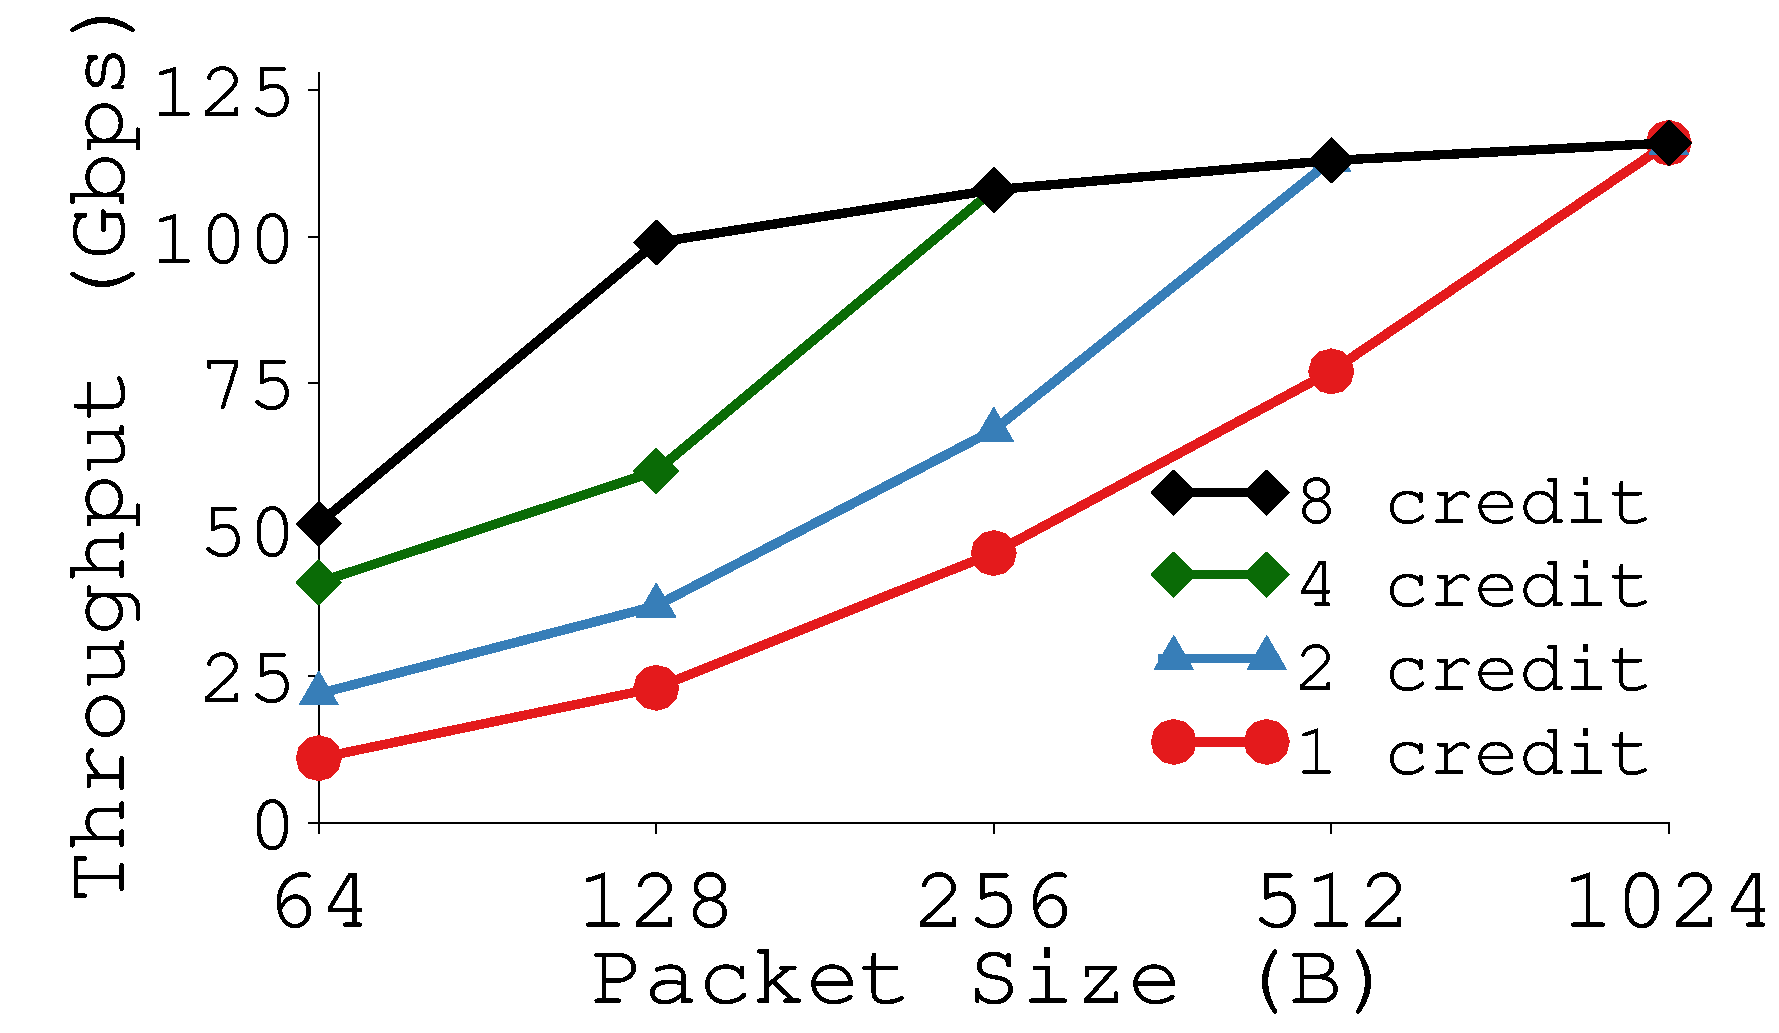
\includegraphics[width=0.5\textwidth]{snic/Figures/g_plot_credit.pdf}}
\mycaption{fig-credit}{Throughput with different credits.}
{
}
\end{center}
\end{figure*}
}
{
\begin{figure*}[h]
\begin{center}
\centerline{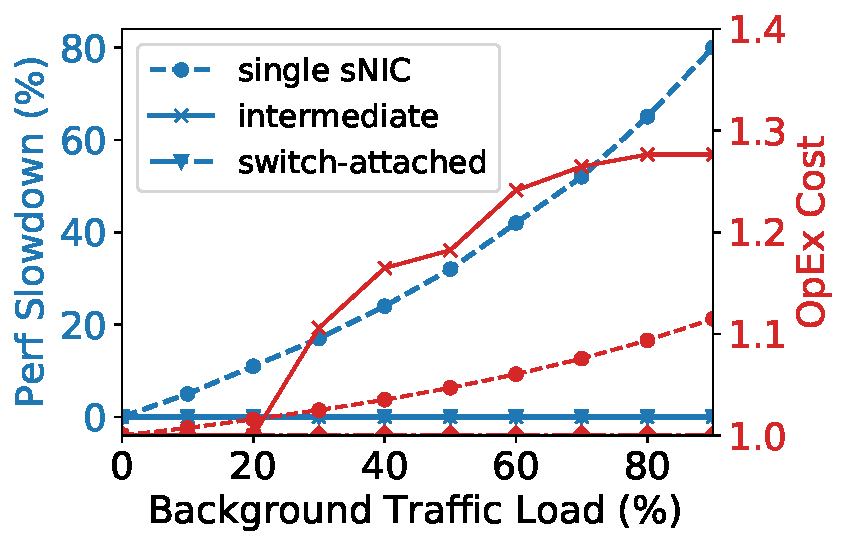
\includegraphics[width=0.5\textwidth]{snic/Figures/fig-dist-nic-load-increase.pdf}}
\mycaption{fig-sim-dist-nic}{Distributed \snic{}.}
{
}
\end{center}
\end{figure*}
}
{
\begin{figure*}[h]
\begin{center}
\centerline{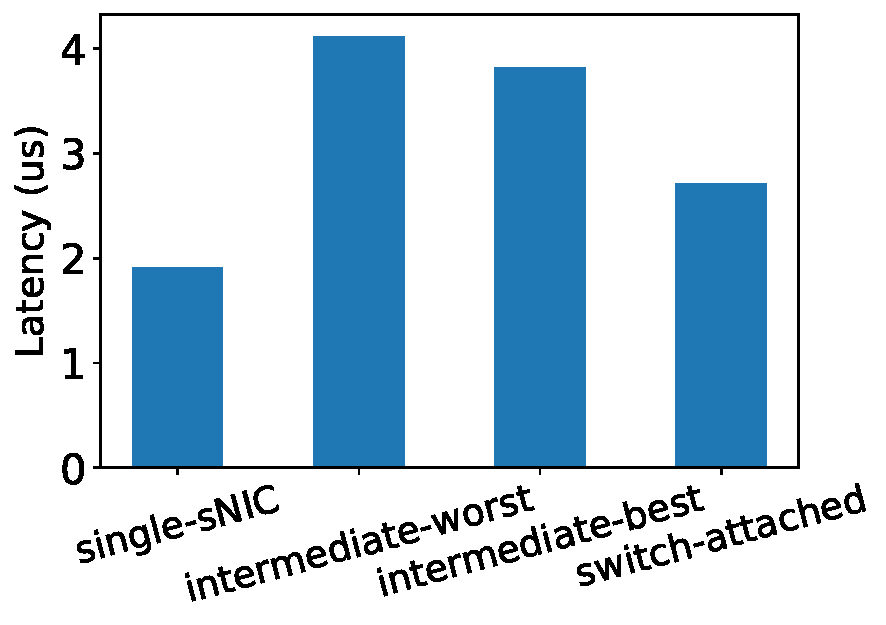
\includegraphics[width=0.5\textwidth]{snic/Figures/fig-dist-nic-latency.pdf}}
\mycaption{fig-topology-cmp}{Topology Comparison.}
{
}
\end{center}
\end{figure*}
}